\documentclass[11pt]{article}

\usepackage{times}
\usepackage{epsf}
\usepackage{epsfig}
\usepackage{amsmath, alltt, amssymb, xspace}
\usepackage{wrapfig}
\usepackage{fancyhdr}
\usepackage{url}
\usepackage{verbatim}
\usepackage{fancyvrb}
\usepackage{float}

\usepackage{subfigure}
\usepackage{cite}
\usepackage{hyperref}
\hypersetup{%
    pdfborder = {0 0 0}
}
\topmargin      -0.50in  % distance to headers
\oddsidemargin  0.0in
\evensidemargin 0.0in
\textwidth      6.5in
\textheight     8.9in 


%\centerfigcaptionstrue

%\def\baselinestretch{0.95}


\newcommand\discuss[1]{\{\textbf{Discuss:} \textit{#1}\}}
%\newcommand\todo[1]{\vspace{0.1in}\{\textbf{Todo:} \textit{#1}\}\vspace{0.1in}}
\newtheorem{problem}{Problem}[section]
%\newtheorem{theorem}{Theorem}
%\newtheorem{fact}{Fact}
\newtheorem{define}{Definition}[section]
%\newtheorem{analysis}{Analysis}
\newcommand\vspacenoindent{\vspace{0.1in} \noindent}

%\newenvironment{proof}{\noindent {\bf Proof}.}{\hspace*{\fill}~\mbox{\rule[0pt]{1.3ex}{1.3ex}}}
%\newcommand\todo[1]{\vspace{0.1in}\{\textbf{Todo:} \textit{#1}\}\vspace{0.1in}}

%\newcommand\reducespace{\vspace{-0.1in}}
% reduce the space between lines
%\def\baselinestretch{0.95}

\newcommand{\fixmefn}[1]{ \footnote{\sf\ \ \fbox{FIXME} #1} }
\newcommand{\todo}[1]{
\vspace{0.1in}
\fbox{\parbox{6in}{TODO: #1}}
\vspace{0.1in}
}

\newcommand{\mybox}[1]{
\vspace{0.2in}
\noindent
\fbox{\parbox{6.5in}{#1}}
\vspace{0.1in}
}


\newcounter{question}
\setcounter{question}{1}

\newcommand{\myquestion} {{\vspace{0.1in} \noindent \bf Question \arabic{question}:} \addtocounter{question}{1} \,}

\newcommand{\myproblem} {{\noindent \bf Problem \arabic{question}:} \addtocounter{question}{1} \,}


\newcommand{\copyrightnotice}[1]{
\vspace{0.1in}
\fbox{\parbox{6in}{
      This lab was developed for the Labtainer framework by the Naval Postgraduate
      School, Center for Cybersecurity and Cyber Operations under sponsorship from
      the DoD CySP program.  This work is in the public domain, and cannot be copyrighted.}}
\vspace{0.1in}
}


\newcommand{\idea}[1]{
\vspace{0.1in}
{\sf IDEA:\ \ \fbox{\parbox{5in}{#1}}}
\vspace{0.1in}
}

\newcommand{\questionblock}[1]{
\vspace{0.1in}
\fbox{\parbox{6in}{#1}}
\vspace{0.1in}
}


\newcommand{\argmax}[1]{
\begin{minipage}[t]{1.25cm}\parskip-1ex\begin{center}
argmax
#1
\end{center}\end{minipage}
\;
}

\newcommand{\bm}{\boldmath}
\newcommand  {\bx}    {\mbox{\boldmath $x$}}
\newcommand  {\by}    {\mbox{\boldmath $y$}}
\newcommand  {\br}    {\mbox{\boldmath $r$}}


\newcommand{\tstamp}{\today}   
%\rfoot[\fancyplain{\tstamp} {\tstamp}]  {\fancyplain{}{}}

\pagestyle{fancy}
\lhead{\bfseries Labtainers}
\chead{}
\rhead{\small \thepage}
\lfoot{}
\cfoot{}
\rfoot{}




\begin{document}

\begin{center}
{\LARGE LDAP}
\vspace{0.1in}\\
\end{center}

\copyrightnotice

\section{Overview}
This lab illustrates the use of LDAP to authenticate users of Linux systems,
such that multiple computers share a single repository of user and group information, including
the passwords that authenticate users.  This strategy allows users and administrators
to manage a single set of credentials that can then be used to access multiple computers. 

\subsection {Background}
The student is expect to have separately learned about the basic elements of Linux
users, groups and authentication, e.g., the /etc/passwd and /etc/shadow files. 
For example, see the {\tt users} lab. 
The student is also expected to have a basic knowledge of the use of Lightweight Directory
Access Protocol (LDAP).

The student is expected to have some familiarity with the Linux command line,
the basics of the file system, and the ability to locate and edit a file.  And some
experience with the Wireshark tool is expected (e.g., the wireshark-intro lab).

\section{Lab Environment}
This lab runs in the Labtainer framework,
available at http://nps.edu/web/c3o/labtainers.
That site includes links to a pre-built virtual machine
that has Labtainers installed, however Labtainers can
be run on any Linux host that supports Docker containers.

From your labtainer-student directory start the lab using:
\begin{verbatim}
    labtainer ldap
\end{verbatim}
\noindent A link to this lab manual will be displayed.  


\section{Network Configuration}
This lab includes a client computer, two servers and
an ldap server shown in Figure~\ref{fig:topology}.
When the lab starts, you will get one virtual terminal connected 
to the client, and one connected to the ldap server.  You will also
get terminals connected to the two servers.

The host names of each component are per the diagram.  The /etc/hosts files
allow use of these host names instead of explicit ip addresses.

The two Linux servers have been configured to use the ldap server to 
authenticate users.  The ldap server has been initially configured
with a single user whose ID is "mike".

The ldap server is configured for the ``example.com'' domain, with
an ldap administrator of ``admin'' whose password is ``adminpass''

\begin{figure}[H]
\begin{center}
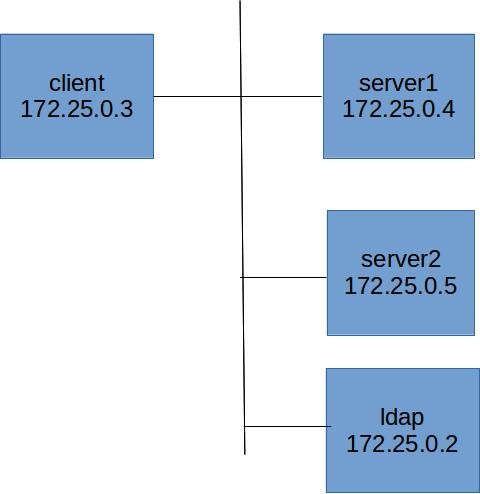
\includegraphics [width=0.8\textwidth]{ldap.jpg}
\end{center}
\caption{Network topology for the LDAP lab}
\label{fig:topology}
\end{figure}

\section{Lab Tasks}
\subsection{Explore}
On the ldap server, display the ldap directory content using:
\begin{verbatim}
   ldapsearch -x | less
\end{verbatim}
\noindent and observe the entries in the directory. Note entry for ``mike'' and
``projx''.

Start wireshark on the ldap component so that you can observe the protocol traffic.
\begin{verbatim}
   wireshark &
\end{verbatim}
\noindent Select the {\tt eth0} device.
From the ``client'' computer, ssh to server1 as user ``mike'':
\begin{verbatim}
   ssh mike@server1
\end{verbatim}
The initial password for ``mike'' is ``password123''.  The system will require that
your change this password and then you will need to ssh again into server1.  Change
the password to whatever you like, but remember it. Use {\tt ssh} again to login to server1
as mike, providing your new password. Use the {\tt id} command to view your user ID
and group. Then,  view the /etc/passwd file.  Do you see entries
for your user or group?

\subsection{View protocol traffic}
Go to the wireshark window, and stop capturing packets (e.g., the red stop button).
Enter a display filter of ``ldap'', i.e., near the top where it says "Apply a display filter...".
Review the LDAP traffic.  Which components are exchanging packets?  Locate the packet that changed
mike's password and use 
\begin{verbatim}
    File / Export Specified Packets 
\end{verbatim}
\noindent to save that packet in a file named {\tt password.pcapng}

\subsection{Use the mike credentials to access another server}
Exit your ssh session from server1.  Then ssh to server2:
\begin{verbatim}
   ssh mike@server2
\end{verbatim}
\noindent What password do you expect to use to authenticate to server2?
After logging into server2, exit that ssh session.

\subsection{Add an LDAP user}
Go to the ldap virtual terminal and use {\tt ls} to see a directory listing.
View the file named {\tt mike.ldif}, it was used to define the user named ``mike''.
Then view the projx.ldif file.
The LDAP command that was used to add the entry defined in mike.ldif is:
\begin{verbatim}
ldapadd -x -W -D "cn=admin,dc=example,dc=com" -f mike.ldif
\end{verbatim}
\noindent Note how the {\tt -D} option names the administrator on whose behalf the
LDAP addition is to be made.  Use {\tt man ldapadd} to learn more about the syntax of
that command. 
The initial password for the mike user was created with this command:
\begin{verbatim}
ldappasswd -s password123 -W -D "cn=admin,dc=example,dc=com" \
   -x "uid=mike,ou=users,dc=example,dc=com"
\end{verbatim}

Create ldif files to define a new group named ``qa'' and a new user having an ID of ``mary''.
Assign mary to the qa group. Take care to adjust the uidNumber and gidNumber values.
Use the ldapadd command to add the new group and the new user.  Use the ldappasswd command to
assign an initial password to mary.  Again, the password for the LDAP administrator is ``adminpass''.

Then go to the client computer and test your ability to ssh as mary to both server1 and server2.

\subsection{Encrypt LDAP traffic}
Go back to the Wireshark window and set the packet display filter to {\tt ldap.bindRequest\_element}.
Explore the protocol elements of one of the bind requests using Wireshark.  See anything alarming?
User passwords are transmitted in plain text!  

Restart the Wireshark capturing, i.e., press the leftmost sharkfin button and clear the filter..

The LDAP server has a self-signed PKI certificate and has been configured to accept encrypted SSL traffic as well as the unencrypted 
traffic that you've observed.  We did not encrypt the traffic to start with so that you could see
the protocol.  You will now configure the LDAP clients (i.e., the two servers) to communicate with
LDAP via SSL.

The mechanisms for causing an LDAP client to use SSL (or TLS) varies by LDAP product and Linux distibution.  For these Ubuntu servers
do the following:

\begin{itemize}
\item Edit the {\tt /etc/ldap.conf} file and change the following line:
\begin{verbatim}
  uri ldap://ldap 
\end{verbatim}
\noindent to
\begin{verbatim}
  uri ldaps://ldap 
\end{verbatim}
\noindent and remove the comment from the line:
\begin{verbatim}
  #ssl on
\end{verbatim}
\noindent so that it is:
\begin{verbatim}
  ssl on
\end{verbatim}
\item Then edit the {\tt /etc/ldap/ldap.conf} file (\textbf{note} the different directory!) and add this line at the end:
\begin{verbatim}
  TLS_REQCERT allow
\end{verbatim}
 
\end{itemize}
No login to one of the servers from the client and observe the LDAP traffic in Wireshark.


\section{Submission}
After finishing the lab, go to the terminal on your Linux system that was used to start the lab and type:
\begin{verbatim}
    stoplab 
\end{verbatim}
When you stop the lab, the system will display a path to the zipped lab results on your Linux system.  Provide that file to 
your instructor, e.g., via the Sakai site.

\end{document}
